\section{Formulación del problema}\label{sec:formulacion}

\subsection{Elementos del modelo}
\begin{table}[H]
\centering\small
\caption{Elementos del modelo.}
\begin{tabularx}{\textwidth}{L{3.6cm}Y}
\toprule
Elemento & Definición \\
\midrule
Instancia & Una empresa/ruta. Las 35 rutas se resuelven por separado y los buses no cambian de ruta. \\
Máquina $i$ & Un bus de la flota operativa de la ruta. Los buses son idénticos en velocidad; solo difieren en su turno de almuerzo. \\
Trabajo $j$ & Una vuelta completa origen $\to$ destino $\to$ origen, con duración base $\pbar_j$ y ventana de inicio $[r_j, d_j]$. \\
Hora de salida $s_j$ & Variable de decisión: instante en que inicia la vuelta $j$. \\
Tiempo de viaje $p_j(s_j)$ & Duración real de la vuelta $j$ si sale en $s_j$, según el perfil de tráfico (sección~\ref{sec:trafico}). \\
Almuerzo & Bloque de 120\,min por bus que inicia en $[a_i, b_i]$: turnos 10:30--11:30, 12:00--13:00 y 13:30--14:30 (el bus $k$ usa el turno $k \bmod 3$). \\
Carga $L_i$ & Suma de los tiempos de viaje de las vueltas asignadas al bus $i$. \\
\bottomrule
\end{tabularx}
\end{table}

\subsection{Origen de los datos}
\begin{table}[H]
\centering\small
\caption{Clasificación de los datos del modelo.}
\begin{tabularx}{\textwidth}{L{4.2cm}Y}
\toprule
Tipo & Contenido \\
\midrule
Datos de la fuente de referencia & Flota operativa, tiempo de vuelta, demanda por hora y viajes por unidad vehicular (tabla de flota operativa 2020). \\
Parámetros construidos por el grupo & Excel del proyecto; vueltas planificadas $=\operatorname{round}(\text{flota} \times \text{viajes por unidad})$; inicios nominales equiespaciados; instancias JSON. \\
Supuestos experimentales & Ventanas de inicio ($\pm15$\,min en 06:00--09:00 y 16:00--19:00; $\pm30$\,min en el resto); jornada de 06:00 a 22:00; almuerzo de 2\,h en tres turnos; perfiles de tráfico T0, T1 y T2. \\
\bottomrule
\end{tabularx}
\end{table}

\subsection{Modelo del tráfico}\label{sec:trafico}
\textbf{$p_j(s_j)$ es el tiempo de viaje (tiempo de procesamiento) de la vuelta $j$ si sale a la hora $s_j$.} El día se divide en franjas $[\tau_k, \tau_{k+1})$ con un factor de congestión $f_k > 0$: dentro de la franja $k$, un minuto real avanza $1/f_k$ minutos del recorrido base. Así, $p_j(s_j)$ es el menor $\Delta$ que cumple:
\begin{equation}
  \int_{s_j}^{s_j+\Delta} \frac{dt}{f(t)} \;=\; \pbar_j .
\end{equation}
Como $f$ es constante por tramos, la integral se resuelve franja por franja hasta completar $\pbar_j$ (Algoritmo~\ref{alg:tiempo}). Se definen tres perfiles:

\begin{table}[H]
\centering\small
\caption{Factores de congestión por franja (parámetros experimentales). T1 = T2 / 1.128.}\label{tab:perfiles}
\begin{tabular}{llccc}
\toprule
Franja & Condición & T2 (pesimista) & T1 (normalizado) & T0 (sin tráfico) \\
\midrule
06:00--06:30 & Valle temprano & 0.90 & 0.798 & 1 \\
06:30--09:00 & Punta mañana & 1.30 & 1.152 & 1 \\
09:00--12:00 & Valle & 1.00 & 0.886 & 1 \\
12:00--14:30 & Punta mediodía & 1.20 & 1.064 & 1 \\
14:30--17:00 & Valle & 1.00 & 0.886 & 1 \\
17:00--20:00 & Punta tarde & 1.35 & 1.197 & 1 \\
20:00--22:00 & Valle nocturno & 0.90 & 0.798 & 1 \\
\midrule
\multicolumn{2}{l}{Media ponderada} & 1.128 & 1.000 & 1 \\
\bottomrule
\end{tabular}
\end{table}

\begin{figure}[H]
\centering
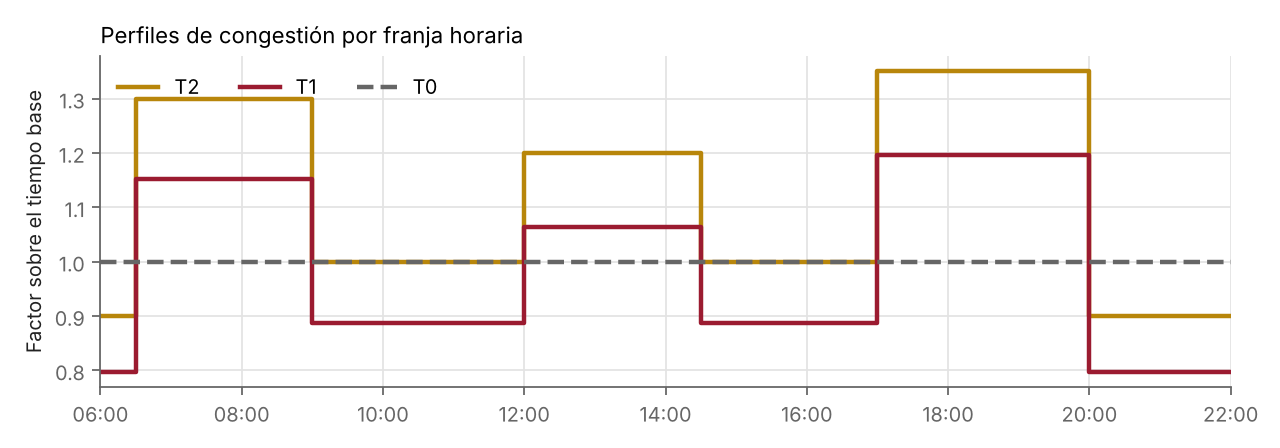
\includegraphics[width=0.85\textwidth]{figuras/fig_perfiles_trafico.png}
\caption{Perfiles de congestión T0, T1 y T2.}\label{fig:perfiles}
\end{figure}

T1 se normaliza para que su media en la jornada sea 1. Así, la duración promedio del día coincide con el tiempo de vuelta de la fuente, que proviene de una velocidad media, y el tráfico solo redistribuye el tiempo entre puntas y valles. T2 representa un día de congestión generalizada (+12.8\,\% en promedio). T0 reproduce el caso sin tráfico.

\begin{nota}
\textbf{\color{guinda}Aclaración.} Los factores de congestión son \textbf{parámetros experimentales} definidos por el grupo; no son mediciones oficiales del tráfico de Cusco. Se almacenan en archivos JSON y en el Excel del proyecto y pueden modificarse sin cambiar el código.
\end{nota}

\subsection{Entradas}
\begin{itemize}
  \item Ruta, empresa y flota $M$.
  \item Vueltas $j$ con duración base $\pbar_j$, salida nominal y ventana $[r_j, d_j]$.
  \item Jornada $[06{:}00, 22{:}00]$ y ventana de almuerzo de cada bus.
  \item Perfil de tráfico (T0, T1, T2 o un archivo JSON).
  \item Algoritmo a ejecutar (LS o LPT).
\end{itemize}

\subsection{Salidas}
\begin{itemize}
  \item Bus asignado, hora de salida y hora de llegada de cada vuelta, o la marca \texttt{NO\_ASIGNADO}.
  \item Hora de almuerzo de cada bus.
  \item Vueltas atendidas, $\Lmax$, cota inferior y brecha, desbalance, utilización y sobrecosto por tráfico.
  \item Resultado de la validación y tiempo de ejecución.
\end{itemize}

\subsection{Restricciones}\label{sec:restricciones}
\begin{enumerate}
  \item \textbf{Ruta:} una vuelta solo se asigna a un bus de su propia ruta.
  \item \textbf{Asignación única:} cada vuelta se asigna a lo sumo a un bus; si no se asigna, queda como no atendida.
  \item \textbf{Ventana:} $r_j \le s_j \le d_j$.
  \item \textbf{Tiempo de viaje:} la vuelta termina en $C_j = s_j + p_j(s_j)$.
  \item \textbf{Jornada:} $s_j \ge 06{:}00$ y $C_j \le 22{:}00$.
  \item \textbf{No solapamiento:} dos vueltas del mismo bus no se superponen.
  \item \textbf{Almuerzo:} cada bus tiene un bloque de 120\,min que inicia en su ventana y no se superpone con sus vueltas.
\end{enumerate}

\subsection{Supuestos}
\begin{enumerate}
  \item Los buses de una ruta son idénticos en velocidad.
  \item La vuelta es indivisible y su duración base es el tiempo de vuelta de la fuente.
  \item En una franja, el tráfico afecta por igual a toda la ruta.
  \item Las ventanas y los turnos de almuerzo son políticas experimentales reproducibles.
  \item No se consideran tiempos de terminal entre vueltas.
\end{enumerate}

\subsection{Formulación matemática y función objetivo}\label{sec:objetivo}
\textbf{Conjuntos.} $I = \{1, \dots, m\}$: buses de la ruta. $J = \{1, \dots, n\}$: vueltas de la ruta.

\textbf{Parámetros.} $\pbar_j$: duración base de la vuelta $j$; $[r_j, d_j]$: ventana de inicio; $[a_i, b_i]$: ventana de inicio del almuerzo del bus $i$; $f(t)$: factor de congestión del perfil; $p_j(s)$: tiempo de viaje de $j$ si sale en $s$ (sección~\ref{sec:trafico}); jornada $[06{:}00, 22{:}00]$.

\textbf{Variables.} $x_{ij} \in \{0,1\}$: vale 1 si la vuelta $j$ se asigna al bus $i$; $u_j \in \{0,1\}$: vale 1 si $j$ no se atiende; $s_j$: hora de salida de $j$; $\ell_i$: inicio del almuerzo del bus $i$.

\begin{align}
  & \textstyle\sum_{i \in I} x_{ij} + u_j = 1 && \forall j \in J \\
  & r_j \le s_j \le d_j && \forall j \in J \\
  & s_j \ge 06{:}00, \quad s_j + p_j(s_j) \le 22{:}00 && \forall j \in J \\
  & a_i \le \ell_i \le b_i && \forall i \in I \\
  & \{[s_j, s_j + p_j(s_j)) : x_{ij} = 1\} \cup \{[\ell_i, \ell_i + 120)\} \ \text{son disjuntos dos a dos} && \forall i \in I \\
  & L_i = \textstyle\sum_{j \in J} x_{ij}\, p_j(s_j), \qquad \Lmax = \max_{i \in I} L_i
\end{align}

\textbf{Función objetivo.} En algunas rutas la flota no alcanza para todas las vueltas, de modo que el objetivo es \textbf{lexicográfico}:
\begin{enumerate}
  \item \textbf{maximizar la cantidad de vueltas atendidas}, equivalente a minimizar $U = \sum_j u_j$;
  \item \textbf{entre las soluciones con el mismo $U$, minimizar $\Lmax$.}
\end{enumerate}
\begin{equation}
  \operatorname{lex\,min}\; \bigl( U,\; \Lmax \bigr)
\end{equation}
Se usa $\Lmax$ y no la hora de fin de la última vuelta porque las ventanas se reparten en toda la jornada: la última vuelta termina cerca de las 22:00 cualquiera sea la asignación, mientras que $\Lmax$ sí mide cómo se reparte la conducción entre los buses.

\textbf{Cota inferior.} Sea $p^{\min}_j$ la menor duración posible de $j$ dentro de su ventana. Para cualquier solución que atienda un conjunto $S$ de vueltas,
\begin{equation}
  \Lmax \;\ge\; LB(S) = \max\Bigl( \max_{j \in S} p^{\min}_j,\; \frac{1}{m}\sum_{j \in S} p^{\min}_j \Bigr).
\end{equation}
La brecha de una heurística se mide contra la cota de las vueltas que atiende.

\subsection{Datos e instancias}\label{sec:datos}
Para la construcción de las instancias experimentales se seleccionaron 35 empresas/rutas de la fuente de referencia que presentan parámetros consistentes para la generación reproducible de las instancias del modelo. El grupo construyó un Excel con esos parámetros; la tabla de flota operativa 2020 es un documento de referencia y no un archivo entregado por las empresas.

Las vueltas de todas las rutas se generan con una misma regla general: el número de vueltas es $\operatorname{round}(\text{flota} \times \text{viajes por unidad vehicular})$; los inicios nominales se reparten de forma equidistante entre las 06:00 y la última salida posible, $\operatorname{round}(22{:}00 - \pbar)$; y cada vuelta recibe una ventana de $\pm15$\,min si su inicio nominal está entre 06:00--09:00 o 16:00--19:00, y de $\pm30$\,min en el resto del día. Las vueltas resultantes se guardan en la hoja \emph{Trabajos y ventanas} del Excel y en una instancia JSON por ruta.

Antes de resolver, el programa regenera las vueltas con esa regla y verifica que coincidan con la hoja del Excel. También comprueba que toda ventana cumpla $r_j \le d_j$, que toda vuelta pueda terminar dentro de la jornada (con tolerancia de 1\,min por el redondeo de las horas al minuto), que los identificadores sean únicos y que la flota no esté vacía. En total hay \textbf{4\,733 vueltas} (entre 103 y 166 por ruta) y \textbf{1\,080 buses} (entre 16 y 44 por ruta).

Para anticipar la dificultad de cada ruta se define la \textbf{saturación} de la flota:
\begin{equation}
  \rho = \frac{\sum_j \pbar_j}{M \cdot 14\,\text{h}} .
\end{equation}
Si $\rho > 1$, la ruta no puede atender todas sus vueltas ni siquiera sin tráfico. Es el caso de RTU-22: 19 buses y 127 vueltas de 2.13\,h requieren 270.5\,h, mientras la flota ofrece 266\,h ($\rho = 1.02$). Las rutas siguientes en saturación son RTI-02 (0.87), RTU-05 (0.82) y RTU-01 (0.79).
